\section{Zadání}

Je dán anonymizovaný dataset o výsledcích léčby pacientů s mozkovou příhodou ve FN Plzeň za 2016-2017.
U pacientů je mimo jiné identifikován etiologický typ mozkové mrtvice, klinický výsledek (škála mRS), míra vstupního deficitu (škála NIHSS), přítomnost rizikových faktorů.
Data nejsou úplná, často jsou některé hodnoty neznámé.

Prvním úkolem je zhodnotit závislosti dobrého klinického výsledku (mRS-out: hodnota 1 oproti 0), případně mortalitu (mRS – 1Y: hodnota 6 oproti 0-5) jednorozměrnou regresí na věku, pohlaví, vstupního NIHSS (TSS příjem) a rozdílu výstupní-vstupní NIHSS.
Druhý úkol spočívá ve vytvoření Kaplan–Meierových křivek přežití pro jednotlivé stanovené diagnózy a podrobně popsat proces vytvoření a její vlastnosti.

\section{Spekulativní exekuce instrukcí}

Spekulativní provádění instrukcí je optimalizační technika, při které počítač (procesor) vykonává dopředu úkoly, aniž by věděl, že budou v budoucnu opravdu potřeba.
To provádí s cílem předejít zpoždění.

Dnešní počítače používají jednu z forem spekulativní exekuce - prediktivní exekuci.
Ta za pomoci mechanismů, jako např. \enquote{branch predictor} odhadne větvení programu a danou cestu předpočítá.
Jestliže se předpověď ukáže jako pravdivá, je \enquote{commitnuta}.
V případě že se ukáže, že předpověď byla špatná, je nutné výpočet zahodit a vykonat správné instrukce.
V případě, že se předpověď prediktoru ukáže jako správná, tak vede ke zrychlení běhu programu.

Dalšími formami spekulativní exekuce jsou např. \enquote{greedy execution} (při které se předpočítají obě možnosti podmíněného větvení) nebo \enquote{lazy evaluation}, která sama o sobě nezahrnuje žádnou spekulaci.
Tyto koncepty se využívají ve světě softwaru a o jejich praktické využití pro hardware jsem se nezajímal.

\section{Meltdown}\label{sec:meltdown}

Moderní operační systémy zajišťují tzv. paměťovou izolaci - uživatelské programy (procesy) nemohou číst z paměťového bloku vyhrazeného pro jiné procesy, obzvláště ne z bloku vyhrazeného pro jádro operačního systému.
\textit{Meltdown} toto omezení zcela překonává a to na hardwarové úrovni.
Útočník napíše kód, který se spustí během spekulativního procesu.
Kód čte data z paměťových bloků, ze kterých nemá práva číst, jelikož ale vše probíhá během spekulativního okna, tak tyto práva jsou teprve kontrolována.
Po dokončení kontroly práv je zjištěno, že program práva na čtení z dané paměti nemá a data jsou zahozena.
Útočník následně provede tzv. \textit{Flush+Reload} útok (\textit{cache side-channel attack}), kterým zjistí nejen kam se zahozená data uložila, ale rovnou i obsah daných paměťových buněk.

Pro útočníka by bylo velice výhodné číst data, které zpracovává jádro operačního systému.
Před zveřejněním diskutovaných hrozeb využíval \textit{Linux} randomizaci adresního prostoru \textit{kernelu (systémového jádra)} (tzv. \textit{KASLR}), ale tento zabezpečovací mechanismus se dal relativně snadno obejít.
Nyní však implementuje vylepšení (tzv. \textit{KAISER} nebo \textit{KPTI}), který zajišťuje, že tabulka indexující uživatelský adresní prostor obsahuje pouze naprosto nezbytné odkazy do adresního prostoru \textit{systémového jádra operačního systému Linux}.
Toto opatření se ukázalo jako dostačující ochrana proti útokům typu \textit{Meltdown}.
Nyní ale systém musí provádět kroky navíc, vždy, když uživatelská aplikace požádá o akci operačního systému (tzv. systémové volání).
Tím se přichází o část výkonu, která je v~některých případech až v řádu desítek procent (z nalezených dat se zdá, že snížení výhonu je ve většině případů \textit{cca} 5 \%, ale ve výjimečných případech může dosáhnout až 30 \%).
Problém s tímto nebezpečím se netýká všech procesorů.
Nejvíce ovlivněným výrobcem (avšak ne jediným) je \textit{Intel}.

\section{Spectre}

V původní práci o útoku typu \textit{Spectre} jsou popsány jeho dvě základní varianty.
Důležitá informace je ta, že na rozdíl od \textit{Meltdown} neumožňuje \textit{Spectre} číst data z celého adresního prostoru, ale pouze z prostoru vyhrazeného pro danou aplikaci.
I tak ale může dojít k odcizení citlivých informací.

\subsection{První varianta}\label{sec:spectre-v1}

První varianta je velice podobná útoku typu \textit{Meltdown}, kdy může útočník při spekulativním vykonávání kódu načíst data na která nemá práva a po jejich zahození je přečíst z \textit{cache} procesoru.

Útočník nechá při trénovací fázi načítat procesor data, která jsou pak použita k lokalizaci jiných dat.
Dotazy na data v rozsahu na která má práva to ale nekončí a útočník se dál dotazuje i na data mimo povolený rozsah.
Procesor v rámci časových úspor načte i data mimo povolený rozsah.
Po zjištění nesrovnalosti procesor data zahodí.

\subsection{Druhá varianta}\label{sec:spectre-v2}

Touto variantou útoku lze natrénovat tzv. \enquote{Branch Target Buffer} tak, že začne provádět kód - \textit{gadget}, jenž bude mít přístup k datům, která jsou předmětem zájmu a která by měla být nepřístupná.
Výsledky jsou opět potlačeny, ale vedlejší účinky provedení daných instrukcí zůstávají.

\section{Foreshadow a další varianty Spectre a Meltdown}

Základními variantami \textit{Spectre} a \textit{Meltdown} problémy s architekturou procesorů bohužel nekončí.
V průběhu roku 2018 přibyly další výzkumy a objevy variant a nových typů zranitelností na \textit{CPU}.
Takovými případy jsou \textit{Foreshadow}, známý též jako \enquote{L1 Terminal Fault (\textbf{L1TF})}, nové varianty \textit{Spetre} a \textit{Meltdown} zmíněné práci \enquote{A Systematic Evaluation of Transient Execution Attacks and Defenses} ale i problémy vzniklé kombinací různých chyb - například \textit{Spectre v2} a \textit{Hyper-Threadingu}.

\begin{quote}
    Problém, o kterém je nyní řeč, se týká využitelnosti chyby \textbf{Spectre v2} v kombinaci s děravým \textit{Hyper-Threadingem} v procesorech \textit{Intel}.
    Ty totiž mají tu nepříjemnou vlastnost, že \textit{HT} vlákna běžící na jednom fyzickém \textit{CPU} jádru sdílejí datovou \textit{L1 cache}, takže za pomoci \textbf{Spectre v2} si může daný proces číst data procesu druhého.
    Do \textit{linuxového} jádra tak zamířily \textit{patche}, které měly tento problém řešit.
    Záplatě se obecně říká \textit{STIBP (Single Thread Indirect Branch Predictors)} a najdeme ji v \textbf{Linuxu 4.20}.
    
    \textit{Phoronix} tuto verzi přeměřil, přičemž dospěl k hodně smutným číslům: záplata snižuje procesorový výkon v mezních případech až o 50 \%, tedy na polovinu.
    Vzhledem k efektivitě \textit{Hyper-Threadingu} v současných \textit{CPU Intelu} lze říci, že výkonnostní dopad aplikace \textit{STIBP} je přibližně stejně dramatický, jako samotné vypnutí \textit{Hyper-Threadingu}.
\end{quote}

\begin{figure}[htbp]
    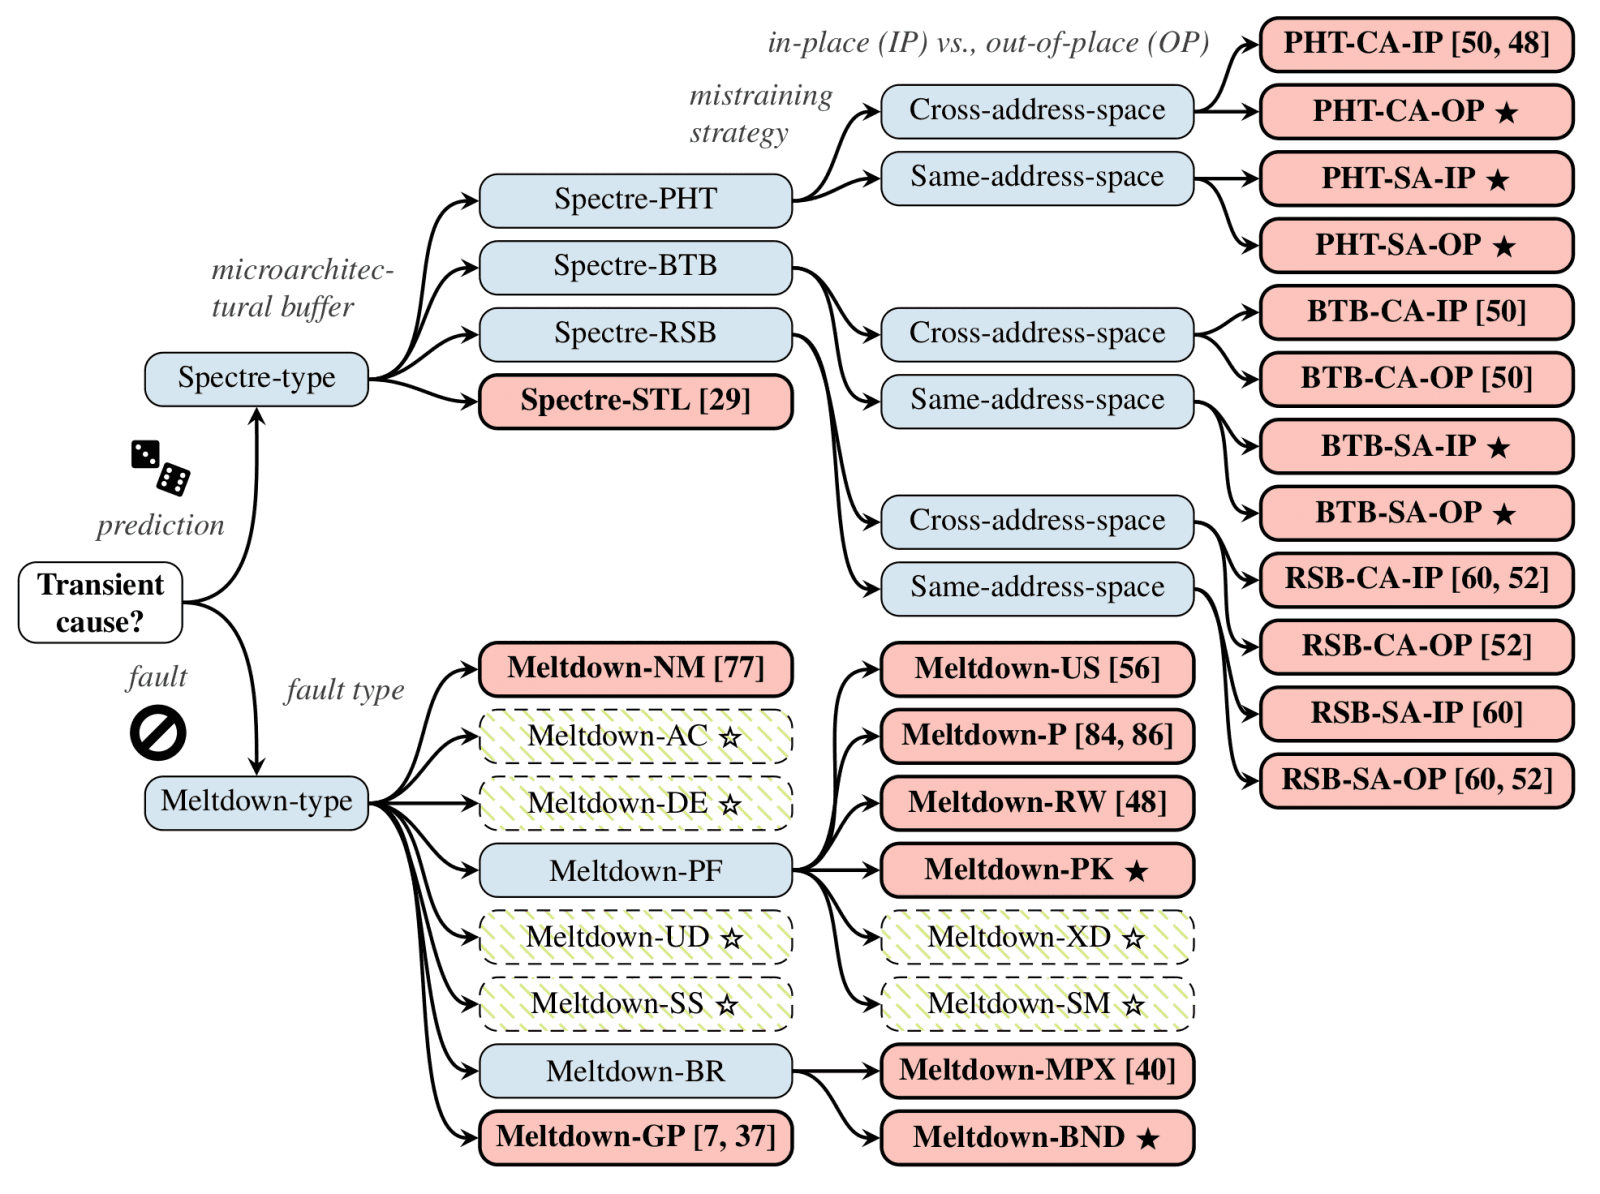
\includegraphics[width=.6\textwidth]{img/klasifikace-spectre-meltdown.png}
    \centering
    \caption{Klasifikační strom s demonstrovanými (červené, tučné), s negativními výsledky (zelené, přerušované) a nově prezentovanými útoky}
    \label{img:klasifikace}
\end{figure}
\FloatBarrier

13. listopadu 2018 byl vydán článek shrnující dosud existující varianty útoků.
Výzkumníci v tomto článku přidali i 8 nových variant útoku \textit{Meltdown} a 5 variant \textit{Spectre} včetně \enquote{proofs-of-concept} pro 7~z~nich - 6 variant \textit{Meltdown} se zatím nepodařilo prakticky dokázat, vše je shrnuto v obrázku \ref{img:klasifikace}.

\subsection{Objasnění pojmů a vztažení nové kategorizace na původní}

Následující výčet pojmů je z převážné části přebrán z článku \enquote{Seven new Spectre and Meltdown attacks found}, ale je doplněn o některá chybějící data.
Tento výčet by měl sloužit jako objasnění, kde se v~nové kategorizaci nachází \textit{Spectre-v1}, \textit{Spectre-v2}, \textit{Meltdown} a také jako přehled s vysvětlením použitých zkratek.

\subsubsection{Kategorizace \textit{Meltdown}}

\begin{itemize}
    \item Meltdown-NM: Floating Point Unit (FPU) state information leakage flaw; linux kernels that follow the "Lazy FPU Restore" scheme are vulnerable to the FPU state information leakage issue; device-not-available exception known as \textbf{\#NM} exception is thrown
    \item Meltdown-AC: tried to exploit memory \textbf{alignment check} exceptions
    \item Meltdown-DE: tried to exploit \textbf{division} (by zero) \textbf{errors}
    \item Meltdown-PF: named after \textbf{Page Fault} \textbf{\#PF} exception
    \begin{itemize}
        \item Meltdown-US: reads kernel memory from \textbf{user space} on pipelined processors that do not transiently enforce the user/supervisor flag
        \item Meltdown-P: attacking faults of pages without \textbf{present} bit
        \item Meltdown-RW: this is in same out-of-order address access of otherwise \textbf{read or write} protected pages, where even content of read or write protected pages could be leaked
        \item Meltdown-PK: bypasses memory \textbf{protection keys} on Intel CPUs
        \item Meltdown-XD: tried to exploit non-executable memory
        \item Meltdown-SM: tried to exploit the \textbf{supervisor mode} access prevention (SMAP) mechanism
    \end{itemize}
    \item Meltdown-UD: tried to exploit invalid opcode exception - Invalid Opcode, known as \textbf{\#UD}
    \item Meltdown-SS: tried to exploit out-of-limit segment accesses - \textbf{Stack-Segment} fault
    \item Meltdown-BR: exploits an x86 bound instruction on Intel and AMD - \textbf{Bound Range} Exceeded
    \begin{itemize}
        \item Meltdown-MPX: MPX stands for \textbf{Memory Protection eXtensions}
        \item Meltdown-BND
    \end{itemize}
    \item Meltdown-GP: \textbf{General Protection} Fault
\end{itemize}

\subsubsection{Kategorizace \textit{Spectre}}

Kategorizace útoků typu \textit{Spectre} je založena na rozlišení toho, který z predikčních mechanismů je využit (\textit{Pattern History Table} (PHT), \textit{Branch Target Buffer} (BTB) nebo \textit{Return Stack Buffer} (RSB)) a který mechanismus se využije k jeho natrénování (\textit{in-place}, nebo \textit{out-of-place}).

\begin{itemize}
    \item Spectre-PHT: exploits the \textbf{Pattern History Table}
    \item Spectre-BTB: exploits the \textbf{Branch Target Buffer}
    \item Spectre-STL: exploits the CPUs memory disambiguation prediction, specifically \textbf{store-to-load} forwarding (STLF)
    \item Spectre-RSB: exploits the \textbf{Return Stack Buffer}
\end{itemize}

\subsection{Negativní výsledky}

Autorům článku \textit{A Systematic Evaluation of Transient Execution Attacks and Defenses} se nepodařilo prokázat uskutečnitelnost útoků souvisejících s načítáním instrukcí do CPU - \textbf{Meltdown-XD} při kterém se pokusili spustit program (instrukce) nacházející v tzv. \textit{non-executable memory} (část paměti obsahující strojový kód, při pokusu o načtení dat z jejího adresního prostoru je vyvolána výjimka) a \textbf{Meltdown-UD} (\#UD - \textit{Opcode exception}) pokoušející se procesor \enquote{donutit} vykonat nevalidní strojové instrukce.

\textbf{Meltdown-SM} nesoucí svůj název podle tzv. \enquote{supervisor mode access prevention} (SMAP) je neúspěšným pokusem o zneužití příznaku udávajícího že určitý program má práva využívat všechny, včetně privilegovaných instrukcí procesoru.

\subsubsection{Meltdown-AC}

\textit{Alignment Check Exception (\#AC)} - v překladu \textit{výjimka kontroly zarovnání} je jedna z výjimek vygenerovaných procesorem při nastání chyby.

Nezarovnaný přístup do paměti (tzv. unaligned memory access) se vyskytne v případě pokusu o čtení N bajtů dat, které začínají na adresní pozici, která není rovnoměrně dělitelná N (tzn. \( adresa \% N \neq 0 \)).
To znamená, že například čtení 4 bajtů dat z adresy 0x10004 je v pořádku, ale čtení 4 bajtů z adresy 0x10005 by znamenalo nezarovnaný přístup do paměti a případné vyvolání výjimky.

Bylo zjištěno, že výsledky nezarovnaných přístupů k paměti nezanechávají data ve struktuře procesoru.
Důvodem je pravděpodobně to, že \#AC výjimka je vygenerována ještě před samotným vykonáváním přístupu do paměti.
Tím pádem varianta Meltdown-AC není zranitelností a není zneužitelná.

\subsubsection{Meltdown-DE}

V článku \textit{A Systematic Evaluation of Transient Execution Attacks and Defenses} byl popsán experiment, při kterém se pokusili získat data, která mohla být teoreticky zanechána v paměti procesoru po vygenerování chyby způsobené dělením nulou.
Podezření se však nepotvrdilo - procesory po dělení nulou vytvoří výjimku (\#DE) a nastaví příslušný registr (paměťový blok uchovávající výsledek operace) na nulu.
Z této operace tedy neexistují žádná zneužitelná data.

\subsubsection{Meltdown-SS}

Posledním z nepotvrzených typů útoků cílí na zneužití \enquote{Stack-Segment Fault} (\#SS).
\textit{Stack-Segment} je dle definice oblast paměti vyhrazená pro automatické proměnné.
Automatická proměnná je lokální proměnná, která je alokována a dealokována automaticky, když tok programu vstupuje a opouští rozsah proměnné.

Jako v předchozích případech, i pokus o přístup do této paměti vyvolá výjimku, k validaci podmínek pro její vyvolání však dochází před samotným přístupem k datům nacházejících se v paměti, kterou se útočník snaží diskreditovat.
Nedochází tedy k žádnému úniku dat.

\subsection{Ostatní útoky typ Meltdown}

\subsubsection{Meltdown-NM}

Popis dle seznamu \textbf{CVE} (\textit{Common Vulnerabilities and Exposures}): \textit{software} využívají metodu pro obnovu stavu \textit{FPU} (\textit{matematického koprocesoru - floating point unit}), tzv. \textbf{Lazy FP} na procesorech od společnosti Intel, může potenciálně umožnit jednomu procesu, aby získal data z jiného procesu přes spekulativní kanál.

Do nedávna byl stav FPU na vyžádání ukládán a obnovován pomocí triku, při kterém použití FPU novým procesem způsobovalo chybu, která spustila logický obvod pro \enquote{save/restore} na samotném matematickém koprocesoru.
Při spuštění nového procesu se využíval starý stav FPU, který byl při prvním opravdovém využití matematického koprocesoru nahrazen správným.
To se dělo s cílem snížit zatížení obvodu pro přepínání úloh.

Starý stav zanechává jistý otisk na struktuře procesoru, který je možné bočním kanálem extrahovat.
Této logiky využívá útok Meltdown-NM.
Tento problém byl na operačním systému Linux vyřešen přechodem na přímé ukládání a obnovu stavu matematického koprocesoru.

\subsubsection{Meltdown-PF}

Meltdown-PF sám spadá do kategorie útoků s \textit{negativními výsledky}, většina jeho podvariant jsou však legitimními útoky.
\enquote{Supervisor Mode Access Prevention} (SMAP) je mechanismus, který zabraňuje procesům s vysokými právy (například procesy operačního systému) číst data z~adresního prostoru procesů patřících uživateli, či jiné entitě s nižšími právy.
Výzkumníci se obávali, že takový přístup mohl zanechat v paměti procesoru data, která by byla přístupná útočníkovi.
Tuto domněnku se nepodařilo potvrdit, jelikož nebyla ve struktuře procesoru nalezena žádná data, která mohla být zanechána po vzniku výjimky.
Stejně jako v případě \textit{Meltdown-AC}, se výzkumný tým domnívá, že výjimka \#PF (page-fault) je vyvolána ještě před vlastní manipulací s daty na fyzických adresních prvcích a tedy neexistují data, která by mohla být ponechána v paměti.

\paragraph{Meltdown-US}

Tato varianta je originálním útokem \textit{Meltdown}.
Pro jeho podrobnější popis viz kapitolu~\ref{sec:meltdown}.

\paragraph{Meltdown-P}

Známý též pod názvem Foreshadow nebo L1TF.
Princip spočívá v tom, že někde v~paměti procesoru se nachází chráněný blok paměti nazývaný \textit{enkláva}.
Když se neautorizovaný požadavek pokusí do této paměti přistoupit, tak není vyvolána výjimka a místo dotazovaných dat se předají data fiktivní.

Díky tomuto mechanismu nefunguje pro získání dat z enklávy klasický útok Meltdown-US.
Tabulka stránek (page-table) tvoří mapování mezi virtuální a fyzickou adresou paměti.
Obsahuje pomocné informace, jako je například \enquote{present} bit, který indikuje které stránky (shluky dat) se nacházejí ve fyzické paměti.

Při útoku \textit{Meltdown-P} se smaže \enquote{present} bit záznamu vedoucího do enklávy, díky tomu lze z tuto paměť načíst aniž by data byla nahrazena fiktivními daty.
Data jsou tedy načtena, ale během jejich zpracovávání procesor zjistí, že došlo k neautorizovanému přístupu, je vyvolána \#PF výjimka a data jsou zahozena stejným způsobem jako při útoku \textit{Meltdown-US}.

\paragraph{Meltdown-RW}

Tento typ útoku je mezi \textit{Meltdown} výjimečný tím, že se nesnaží získat data napříč úrovněmi privilegovaného režimu procesoru, ale překonává zabezpečení na dané bezpečnostní úrovni.
Bylo zjištěno, že při spekulativním vykonávání instrukcí je ignorován příznak umístěný na \textit{tabulce stránek} určující práva pro čtení a~zápis.
Útočník může tím pádem přepsat data určená jen pro čtení, čímž je zcela překonán softwarový bezpečnostní mechanismus zvaný \enquote{sandbox}, který se spoléhá na hardwarové vymáhání přístupu k datům určeným pouze pro čtení.

\paragraph{Meltdown-PK}

Tímto útokem lze číst data chráněná technologií Intel Protection Keys.
Varianta byla prezentována a dokázána v článku \textit{A Systematic Evaluation of Transient Execution Attacks and Defenses}.

\textit{Intel Protection Keys} je technologie nacházející se na některých procesorech od společnosti \textit{Intel} umožňující uživatelským procesům měnit práva tomuto procesu náležícím stránkám v tabulce stránek.
To má za cíl umožnit vývoj bezpečnějších aplikací.
Zajímavé je, že proti tomuto útoku neexistuje softwarová záplata - pokud uživatelský program používá \textit{Intel Protection Keys}, tak je zranitelný.
Chybu musí opravit \textit{Intel} v nové verzi procesorů.

\subsubsection{Meltdown-BR}

Pro efektivní vývoj softwaru procesory poskytují nástroje jako je například výjimka \textit{bound range exceeded (\#BR)} upozorňující na iterování přes indexy mimo pole.
\textit{Meltdown-BR} poskytuje způsob, jak obejít kontroly na procesoru, které vyvolávají \#BR výjimku.
Tím je umožněno číst data za povolený rozsah odpovídající velikosti iterovaného pole a získat tak informace, ke kterým za normálních okolností nemá útočník přístup.

O variantách \textbf{Meltdown-MPX} a \textbf{Meltdown-BND} se mi nepodařilo zjistit dostatek informací, abych o nich mohl podrobněji referovat.
O \textbf{Meltdown-MPX} pojednává původní článek vydaný Intelem, k \textbf{Meltdown-BND} jsem materiál nenalezl.

\subsubsection{Meldown-GP}

Tato varianta umožňuje útočníkovi číst data z registrů procesoru vyhrazených pro operační systém.
Bylo zjištěno, že ačkoliv je po pokusu o přístup do takové paměti vyvolána \#GP (\textit{general protection fault}) výjimka, jsou data i přesto dostupná v případě, že výjimka vyvstala při spekulativním vykonávání instrukcí.
Za normálních okolností nepřístupná data o systému mohou být získána postranními kanály (např. již zmíněným útokem \textit{Flush+Reload}).

\subsection{Útoky typu Spectre a pojmy}

\begin{figure}[htbp]
    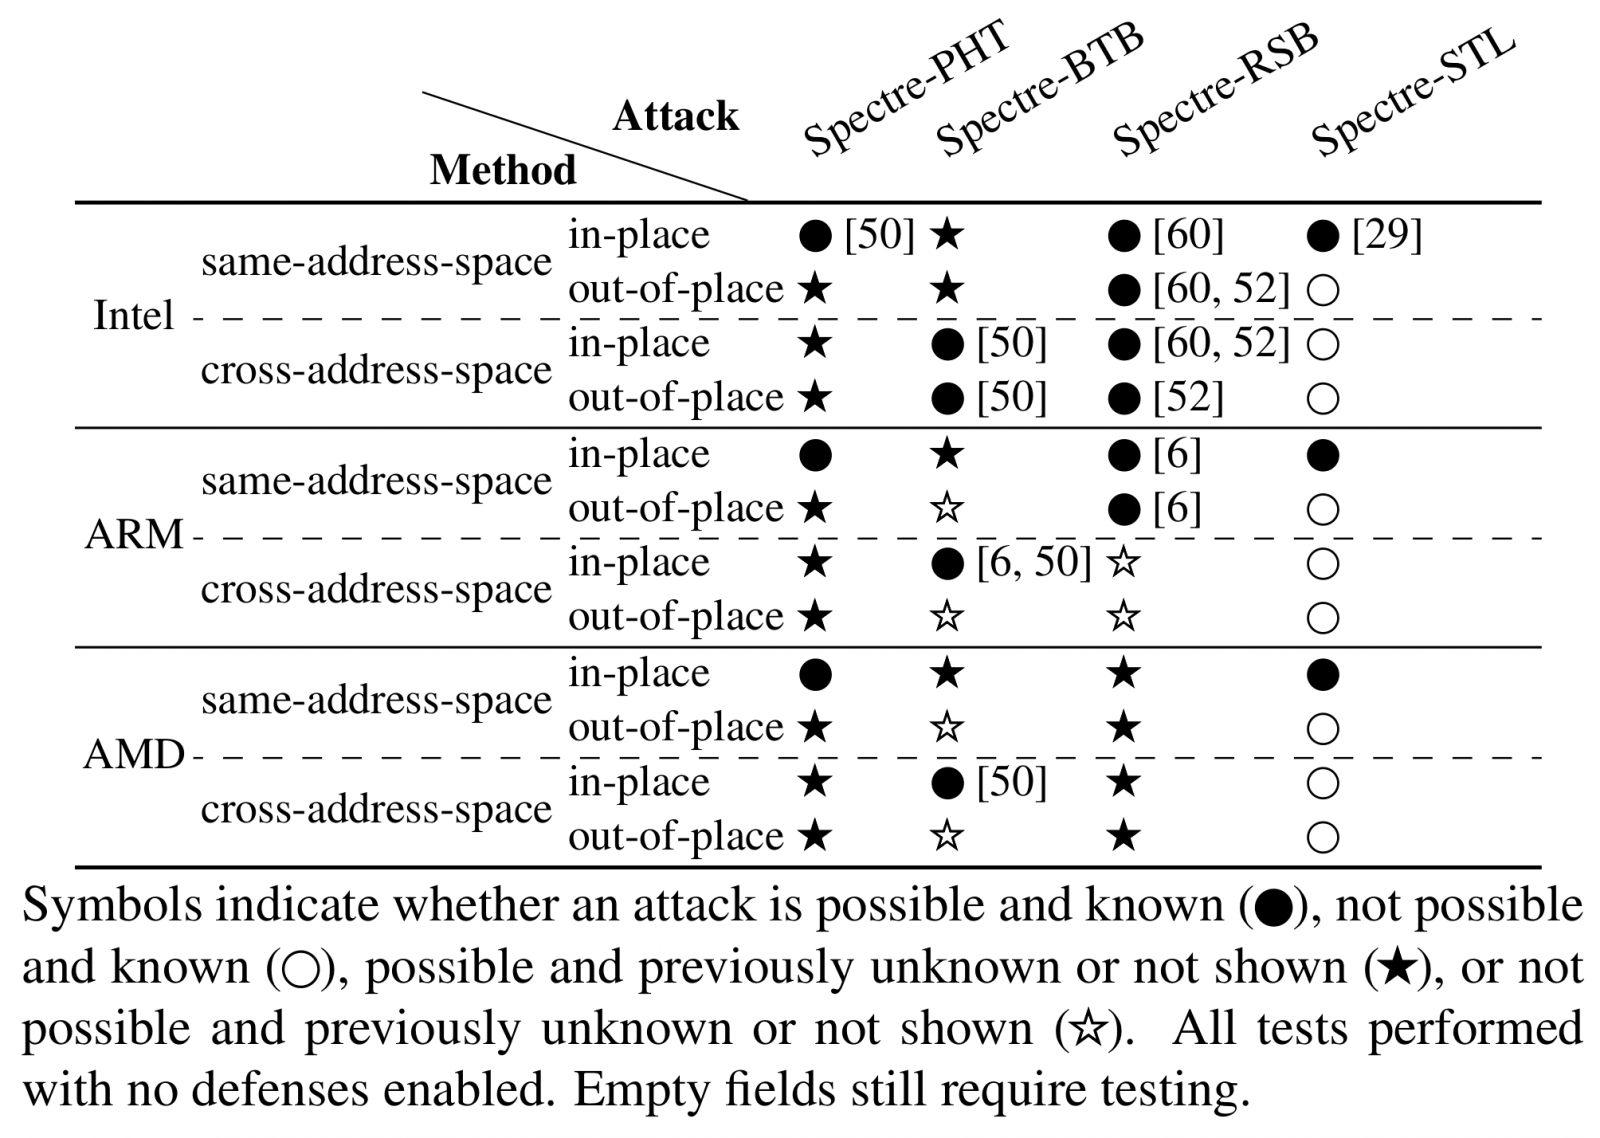
\includegraphics[width=.8\textwidth]{img/spectre-1.png}
    \centering
    \caption{Shrnutí variant Spectre, jejich známosti, adresního prostoru na který je možno útočit a~ovlivněný výrobce/architektuar procesorů.}
    \label{img:spectre}
\end{figure}
%\FloatBarrier

\subsubsection{Spectre-PHT}

PHT (Pattern History Table) je struktura sloužící jako prediktor výsledků operací.
Tato struktura (tabulka) je předtrénována tak, aby načetla načetla data, na která nemá útočník právo.
Tento útok je originální variantou útoku \textit{Spectre-v1}.

\subsubsection{Spectre-BTB}

Originální útok \textit{Spectre-v2}.
\enquote{Branch Target Predictor} je část procesoru, která předpovídá výsledek kódu nacházející se v podmínkové větvi programu.
\enquote{Branch Target Buffer} (BTB) je vyrovnávací paměť, která uchovává výsledky, na rozdíl od \textit{PHT} je ale separátní pro každou podmíněnou větev.
Na rozdíl od Spetre-PHT, kde útočník přetrénuje mechanismus validními hodnotami, Spetre-BTB přetrénuje mechanismus vlastními škodlivými daty.
Díky tomu si útočník může navolit data tak, že směřují na paměť obsahující tzv. \enquote{gadget}, což je kód, který se spustí a vystaví útočníkovi původně tajné informace (přenese data do kanálu, který je plně v režii útočníka).
Aby bylo možné takový útok provést, tak musí být známa virtuální adresa \enquote{gadgetu} v adresním prostoru.

\subsubsection{Spectre-STL}

Dalším způsobem, jak zlepšit výkon procesoru je zápisu aktualizovaných výsledných hodnot do vyrovnávací paměti namísto zápisu přímo do paměti k tomu určené (např. cache nebo RAM).
Bez této nutnosti neustále načítat a ukládat data do pomalejší paměti je umožněno procesoru provádění pokynů v rychlejším tempu.
Všechna data uložená v zásobníku se nakonec zapíšou zpět do hlavní paměti.
Při takovém procesu vzniká riziko, že je přečten obsah vyrovnávací paměti před tím, než stačí být zapsána aktualizovaná hodnota.
Aby se této situaci zabránilo, procesor kontroluje vyrovnávací paměť před každým čtením, které provádí.
Při těchto operacích je povolen \enquote{unaligned access} (nezarovnaný přístup) do paměti a tak je celý proces kontroly výpočetně náročný.
Tento proces je nazýván \enquote{disambiguace paměti}.

Jelikož je proces kontroly vyrovnávací paměti náročný, tak se používá další urychlení - \enquote{Speculative Store Buffer Bypass}.
V případě, že process disambiguace předpoví, že načítání nebude kolidovat s~ukládáním dat do vyrovnávací paměti, tak není kontrola vyrovnávací paměti prováděna.

Optimalizace \enquote{Speculative Store Buffer Bypass} byla v kombinaci s \enquote{Flush+Reload} útokem zneužita k získání hodnot z vyrovnávací paměti.
Omezením \textit{Spectre-STL} (\textit{Speculative Store Bypass}) je, že útočník může získat informace pouze z paměti, která se nachází na stejné úrovni privilegovanosti jakou má program využitý k útoku.

\subsubsection{Spectre-RSB}

Na rozdíl od předešlých útoků, Sperctre-RSB nezneužívá prediktory větvení (branch predictors), ale \enquote{Return Stack Buffer}.
\textit{RSB} je lokální, při změně kontextu resetovanou, kopií struktury \enquote{Call Stack}, obvykle o velikosti 4~-~16 záznamů.
\enquote{Call Stack} je datová struktura uchovávající informace o~aktivních subprocesech počítačového programu.

Příkaz \textit{return} v počítačovém programu obvykle vrací vypočtenou hodnotu funkce do místa, odkud byla funkce zavolána.
Kam má hodnotu vrátit dohledává ve struktuře \textit{call stack}.
Aby bylo nalezení cílové lokace rychlejší, tak se používá menší kopie - \textit{RSB}.

Ve článku \textit{Spectre Returns! Speculation Attacks using the Return Stack Buffer} je prezentováno několik variant útoku na \textit{RSB} s cílem získat data která nemají být přístupná.

První varianta je způsobené přehlcením \textit{RSB}, to způsobí přepsání skutečných užitečných adres, na které by mělo být referováno, ale už nemůže být, protože se v \textit{RSB} nenachází.

Druhá varianta upravuje hodnoty v \textit{RSB} napřímo - ať už je přepisuje nebo rovnou maže.
To způsobuje neshodu mezi hodnotami v \textit{RSB} a \textit{call stacku} a tudíž mispredikci procesoru.

Třetí varianta naplňuje \textit{RSB} adresami, které jsou mimo povolený adresní prostor.
Ostatními okolnostmi popisovanými v originálním článku je pak možno na tyto adresy přistupovat bez vyvolání výjimek procesorem.

Čtvrtá varianta zahrnuje sdílení \textit{RSB} napříč vlákny CPU bez resetování hodnot při kontextuálním přechodu.

\section{Závěr}
